\subsection{Structure of the section}
Overview stating the goals we want to convey through the experiment section. The what and how of the experiments.
\section*{Experiments}
\subsubsection*{Overview}
In this chapter, we perform various qualitative and quantitative evaluations to showcase a comprehensive performance comparison of our method to others. All the experiments are conducted in the in-house built simulator described in Section \ref{section}. There are a lot of choices regarding methods and features that have been made, and we try to evaluate each of these choices against the existing work.\\
The first subsection provides a comparison among our IRL method, a classical agent, and an RL based agent trained in a similar setting using a simple yet dense hand-crafted reward function. This helps in demonstrating the difference in the performance of agents coming from different training methods.\\
 Feature representations play a vital role in an IRL pipeline and so, the following section compares the performance of IRL agents trained in a similar setting but different feature representations.\\
This is followed by a set of experiments to evaluate the generalizability of our setup, where the performance of an agent is compared between a known and an unknown environment. Here "known" is defined as the environment from which the expert demonstrations have been collected.\\

Getting tricky scenarios that help showcase the subtle qualitative aspects of a navigating agent from the real-world video might be difficult and indeed with the time and effort spent scrolling through the videos to find these are hard, so we also generate some synthetic scenarios to check some of the specific, more advanced qualitative behaviors of the IRL and how that differs to that of the RL.

The last subsection looks into the reward function: the second, and unfortunately, in most of the cases, ignored part of the equation. We try to visualize and interpret the reward function in an attempt to get a better insight into the functioning of our agent.

\subsubsection*{Description of the scenario}
To train our agent we select demonstrations from the UCY university students dataset \cite{ucy-dataset-university-students}. It consists of trajectories of 430 different pedestrians on a relatively busy area captured over 3 minutes and 37 seconds. The video is captured at 25 fps resulting in a total of 5400 frames. The length of the trajectories varies from $the min$  to $the max$ with an average of 406 frames per trajectory. 
\begin{figure}
    \caption {Distribution of pedestrian trajectory length}
\end{figure}
There are a few key properties that make this environment challenging: dense crowd, open space so lack of any constrain offered by spaces like narrow pathways, as because open space pedestrians(obstacles) can and does come from different directions making the process of negotiating such crowds rather challenging. 

%\begin{table}
%    \caption {Table containing useful information on the what is useful}
%    \label{university-students-stats}
%        \begin{center}
%        \renewcommand{\arraystretch}{1.3}
%        \begin{tabular}{|c|c|}
%            \hline
%            Property  & Value \\
%            \hline
%            Number of pedestrians &    \\
%            Avg trajectory length &  \\
%             & $\theta > 90\degree$\\
%            
%            Medium & otherwise \\
%            \hline
%        \end{tabular}
%    \end{center}
%\end{table} 
\subsubsection*{Description of the training parameters?}

The MEDIRL pipeline is run for 100 epochs. The AC2 \cite{ac2} training for the inner loop is run for a predefined fixed number of episodes where an episode terminates when the agent reaches the goal, hits an obstacle, or exceeds a predefined maximum number of frames per episode. Both the policy and reward networks have a simple architecture with a single 256-dimensional hidden node with an exponential linear unit (ELU) \cite{exponential-linear-unit} as the activation function and adaptive moment estimation (Adam) \cite{adaptive-moment-estimation} as the choice of the optimizer. The learning rate for the policy and reward network is set to $0.001$ and $0.0005$ respectively.


\subsubsection*{Description of the metrics used}
%What do we want to show? 
%\begin{enumerate}
%    \item Justify the use of IRL over RL or traditional methods.
%    \item Establish the superiority of the feature representation over other
%    \item Show that the smoothing affects the performance of the agent in a positive way.
%    \item Show the generalizability of the method. (Compare the performance metrics of the agent in the two different scenarios.)
%    \item Another benefit of IRL is the availability of the reward network. Visualization and comprehension of the reward network. 
%\end{enumerate}
%How do we show?
%
%To test the generalization capabilities of our method we train on the expert demonstrations from lone of the video and test it on data from different scenarios.

%\begin{itemize}
%        \item Training and testing on the same annotation file.
%        \item Training and testing on different annotation files.
%        \item Testing on custom scenarios.
%\end{itemize}
To get a comprehensive comparison of the performance of the agents, we compare them among different metrics, each capturing a unique characteristic of the navigation behavior exhibited by the agent. The metrics are described below:
\begin{itemize}
        \item \textbf{Reaching the goal:} The ability to reach a goal from a given position is one of the fundamental criteria to measure the performance of a navigating agent. It is calculated as the percentage of runs per 
        \item \textbf{Distance to displacement ratio:} This metric captures the efficiency of the path an agent takes to move between two points. It is calculated as the ratio between the euclidean distance between the two points and the distance traveled by the agent to move between the two. So, for two agents moving from the same start and endpoints, given both of them are successful in reaching the goal, the agent taking a more direct path, is rated better than the other. (The results are shown in the form of histogram plots)
%        \item \textbf{Minimum distance over time graphs:} Indicates the minimum distance maintained by an agent throughout its entire trajectory. It can be thought of as a measure of how 'dangerously' or 'cautiously' an agent behaves while interacting with neighboring obstacles. (line graphs over time frame)
        \item \textbf{Avg smoothness:} Trajectories traced by people are smooth with rare occurrences of drastic change in the heading direction. This metric measures how much an agent changes its heading direction, thus the smoothness of its trajectory while negotiating obstacles or navigating in general. (bar plots with error bars.)
        \item \textbf{Drift analysis plots: }The main aim of the project is to obtain intelligent agents that navigate and interact with crowds humanly, which is why the drift analysis is one of the most important metrics we use to evaluate the agents. This performs a direct comparison between the trajectory taken by an agent and the trajectory followed by the pedestrian and is calculated as the MSE between the points on the trajectory of the agent and the pedestrian(ground truth)at each time frame. The comparison is performed over a range of trajectory segment lengths with an aim to showcase the short to medium term navigation capabilities of the agents. It is a measure of how much the trajectory traced by an agent conforms to the original trajectory of the pedestrian when subjected to similar conditions. (line graphs with error bars)\\
        \textbf{\textcolor{red}{Navigation is an under-constrained problem}}, some more that others. This is especially true for cases where are not a lot of obstacles around and there is more that one way to reach the goal from a given position which are just as good. To better understand the 'drift' of the agents from the ground truth pedestrians, we classify the pedestrians into 3 different classes: easy, medium and hard, based on the number of pedestrians nearby throughout the trajectory and perform separate drift analysis on the pedestrians of each class. \textcolor{red}{the criteria for classification}. The idea is that, a pedestrian from the 'easier' class encounters relatively less crowd along its path, which in turn provides a wider choice of 'good' trajectories, that does not necessarily conforming to the original ground truth. 
        \item \textbf{Traced trajectory of multiple agents for a particular pedestrian:} Primarily a visual tool to see how an agent performs in comparison to the ground truth.
\end{itemize}

\section*{Results and discussion}
\subsection*{Testing the performance against other methods}
In this section we compare an agent trained using our IRL pipeline to two different agents: a data driven RL agent and a model based potential-field controller. The RL agent is trained in the same environment as the IRL using similar training hyper-parameters and network architecture with a dense reward function shown in Table  \ref{tab:reward-function-summarization}.
\begin{table}[htbp]
    \caption{Summary of reward function for RL agent}
    \begin{center}
        \renewcommand{\arraystretch}{1.3}
        \begin{tabular}{|c|c|}
        \hline
        Condition & Reward assigned \\
        \hline
        Reach goal & 1 \\
        Hit obstacle & -1 \\
        Move towards goal & $0.01 \times \text{length of the step}$ \\
        Move away from goal & $ -0.01 \times \text{length of the step}$\\
        \hline
        \end{tabular}
    \end{center}
    \label{tab:reward-function-summarization}
\end{table}\\
The implementation of the potential field controller is based on \cite{khatib-potential-field}.\\  
\begin{figure}[htbp]
    \begin{subfigure}{0.5\textwidth}
        \centering
        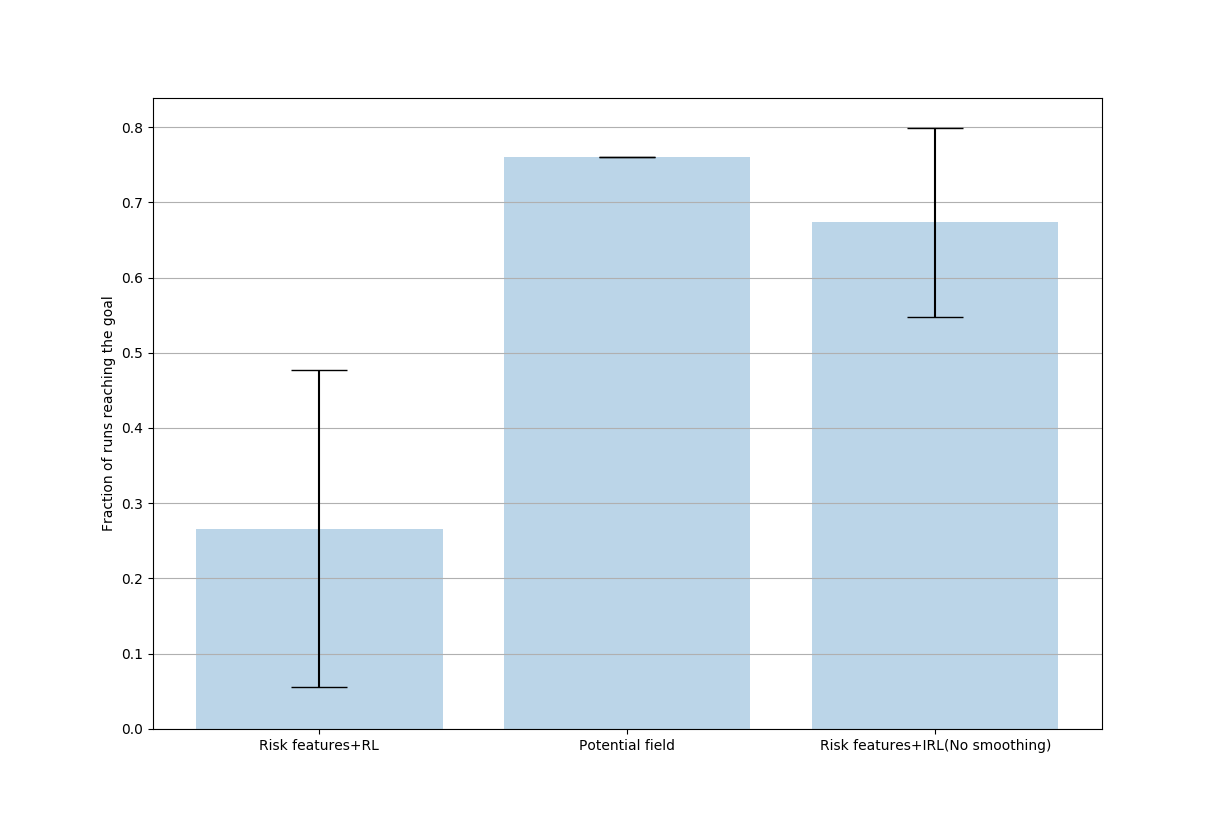
\includegraphics[width=0.95\linewidth, height=6cm]{plots/inter_method/goal_reached.png}
        \caption{A comparison of the fraction of successful run completions of agents trained using 3 different methods.}
        \label{fig:inter_method-goal_reached}
    \end{subfigure}
        \begin{subfigure}{0.5\textwidth}
            \centering
        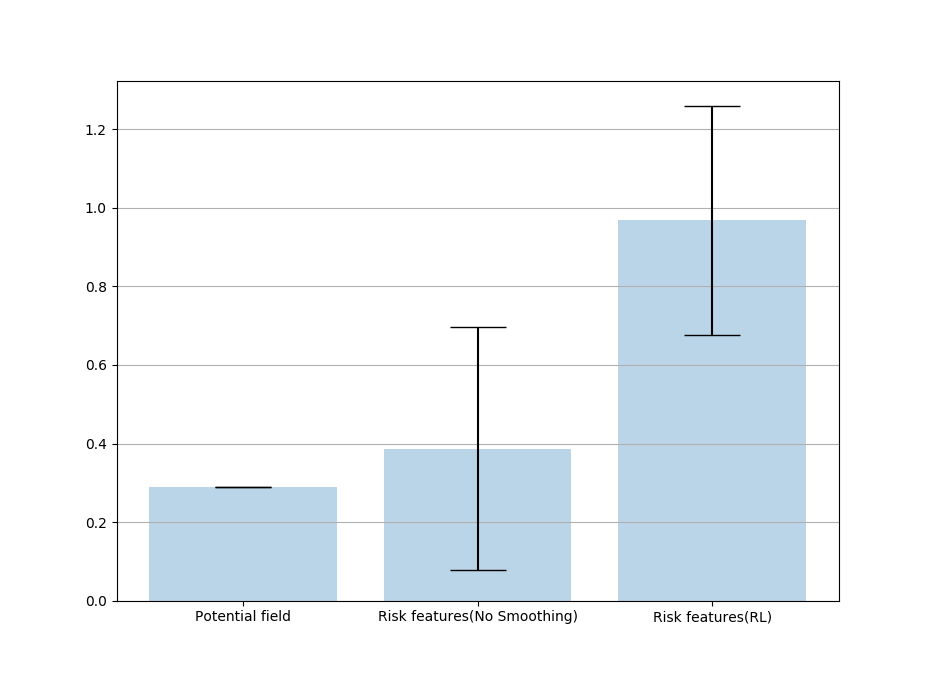
\includegraphics[width=0.95\linewidth, height=6cm]{plots/inter_method/collision_counts.png}
        \caption{A comparison of the fraction of successful run completions of agents trained using 3 different methods.}
        \label{fig:inter_method-collision_counts}
    \end{subfigure}
\caption{Comparing the fundamental properties of navigation in agents trained using different methods}
\end{figure}\\

Figure \ref{fig:inter_method-goal_reached} and \ref{fig:inter_method-collision_counts} show that out of the 3 agents, the potential field and the IRL based method are significantly better at navigating the environment with potential field slightly pulling ahead of the IRL agent in both the criteria. In the task of reaching the goal, the potential field achieves a success rate of $78.37\%$ closely followed by the IRL agent with a success rate of  $74.49\%$ and finally, the RL agent with $35.58\%$. The average number of collisions encountered by the agents also has a similar trend, with the PF agent encountering the least number of collisions at $0.29$ per trajectory, followed by the IRL agent and the RL agent at $0.39$ and $0.97$ respectively. This is understandable for a PF controller as they are explicitly designed to reach a goal in conjunction with collision avoidance, and with the absence of local-maxima, which is one of the major drawbacks of the method, the potential field agent is at its niche. It is also interesting to see that opting for IRL over RL as the choice of training significantly increases the objective performance of the agent.

%Figure \ref{fig:inter_method-reach_goal}, and \ref{fig:inter_method-collision_counts} shows that both, the IRL agent and the potential field controller are better at avoiding obstacles when compared to the RL agent, with the potential field controller having a slight edge over the IRL agent in both the cases. This is somewhat understandable as we know that classical methods like potential fields are potent navigation algorithms. Although it has its drawbacks, including but not limited to the inability to negotiate local minima, the highly dynamic environment rarely presents one.  

\begin{figure}[htbp]
    \centering
    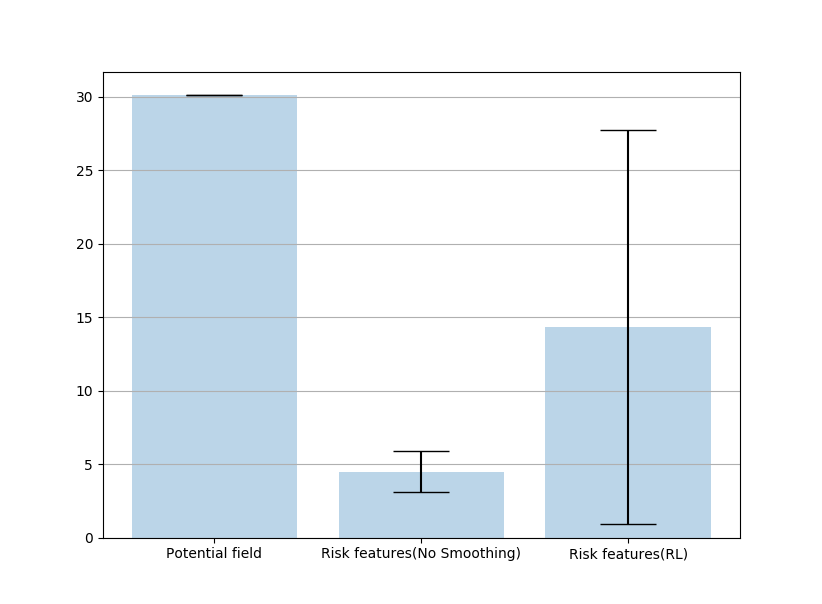
\includegraphics[width=0.7\linewidth]{plots/inter_method/trajectory_smoothness.png}
    \caption{Average change in orientation of different agents.}
    \label{fig:inter_method-change_in_orientation_avg}
\end{figure}
While PF agents are good navigators, their movement patters are not the smoothest, as slight change in the configuration of the nearby obstacles can significantly change the potential field around it. This is reflected in Figure \ref{fig:inter_method-change_in_orientation_avg}, where the PF agent, on average, changes its orientation by almost $30.14\degree$ per frame compared to the $14.33\degree$ of the RL agent and insignificant $4.48\degree$ of the IRL agent.

\begin{figure}[!htbp]
    \begin{subfigure}{\textwidth}
        \centering
        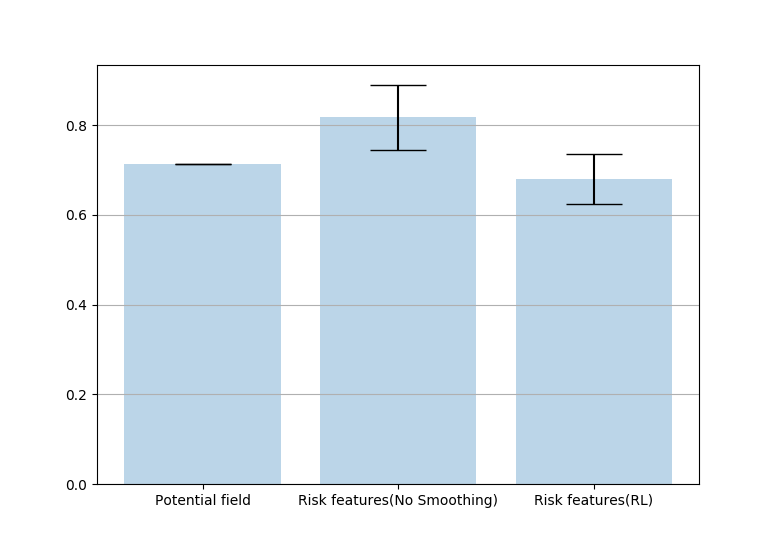
\includegraphics[width=.7\linewidth]{plots/inter_method/distance_displacement_ratio.png}
        \caption{Histogram plot of distance displacement ratio.}
        \label{fig:inter_method-distance_disp_ratio}
    \end{subfigure}
    \begin{subfigure}{\textwidth}
        \centering
        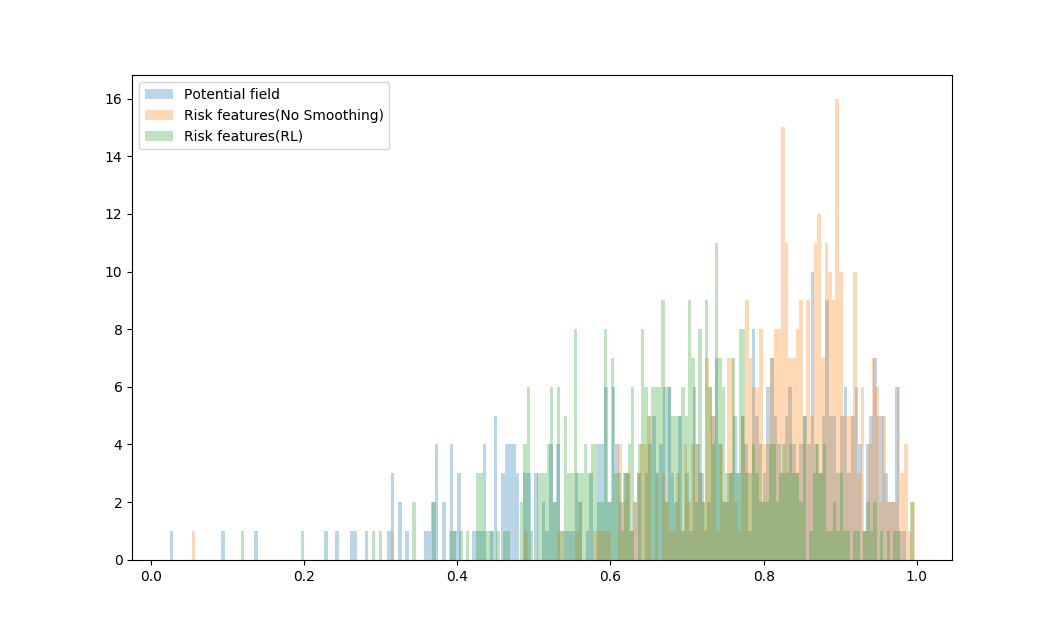
\includegraphics[width=.95\linewidth]{plots/inter_method/histplot_displacement_ratio.png}
        \caption{Histogram plot of distance displacement ratio.}
        \label{fig:inter_method-distance_disp_ratio_histplot}
    \end{subfigure}
    \caption{Comparing the efficiency of the path taken by the different agents to reach their goals}
\end{figure}
Figure \ref{fig:inter_method-distance_disp_ratio} shows that the IRL agent tends to produce more effective trajectories at a distance-displacement ratio of $0.81$ as compared to the $0.71$ and $0.67$ of the PF and RL agent respectively. Figure \ref{fig:inter_method-distance_disp_ratio_histplot} provides a more detailed insight on the distribution of the same over all the trajectories. It shows that for the IRL based agent most of the runs are clustered around the range of $0.8 - 0.9$, and while the PF agent does have a higher density in the range of $0.9 - 1.0$, its distribution is spread over a wider range, with significant number of samples in the sub $0.5$ range. The RL agent on the other hand has a distribution similar to that of the IRL, but with the mean more towards the mid $0.70s$. Table \ref{tab:inter_method_numerical_results} shows a comparison of the different methods.
\begin{table}[htbp]
	\begin{center}
		\renewcommand{\arraystretch}{1.3}
		\begin{tabular}{|c|c|c|c|c|}
			\hline
			Metric Name & Potential Field & RL & IRL  &  Ground Truth \\
			\hline
			Goal reached (in $\%$) & $78.37$ & $35.58$ & $74.49$ & $91.16$\\
			Collisions encountered (per run) & $0.29$ & $.96$ & $0.38$ & $0.10$\\
			Change in orientation ( $\degree$ per frame) & $30.14$ & $14.33$ &  $4.48$ & $1.14$ \\
			Displacement to Distance ratio & $0.71$ & $0.67$ & $0.81$ & $0.84$ \\
			\hline
		\end{tabular}
	\end{center}
	\caption{Score obtained by the different feature representations across different metrics}
	\label{tab:inter_method_numerical_results}
\end{table}\\
\textbf{Drift analysis}\\
\textcolor{red}{Figure \ref{fig:inter_method-drift_analysis_all} shows that the IRL agent suffers the least amount of drift when calculated over the set of all the pedestrians. The results from the pedestrian groups of varying difficulty provides more insight. The amount of drift suffered by the agents is inversely proportional to the difficulty level of the pedestrian trajectory as shown in Figures. \ref{fig:inter_method-drift_analysis_easy}, \ref{fig:inter_method-drift_analysis_med}, \ref{fig:inter_method-drift_analysis_hard}. This is understandable, as the clutter around a pedestrian decreases, the agent has less incentive to follow that 'one' path traced by the original pedestrian as a scant crowd increases the option of available good paths. As the difficulty increases, the room for taking good alternative trajectories decreases and so does the drift, with the IRL agent being the quickest to conform to the expert trajectory not only displaying the least drift suffered but also producing the biggest reduction.}\\
\vspace{5cm}
%
%As the difficulty increases, all the agents show reduced drift, with the IRL agent enjoying significantly lower values as compared to the other. This implies that the rate of resemblance.
%An extreme case on the opposite spectrum would be when only one single trajectory is a collision free path that reaches the goal, in that case, all the successful agents should follow the exact trajectory traced by the pedestrian. For all the in-between cases, successful trajectories can be classified into ones that conform to pedestrians and not. Our method conform more to the pedestrians as compared to the rest.
\begin{figure}[htbp]
	\begin{subfigure}{0.5\textwidth}
		\centering
		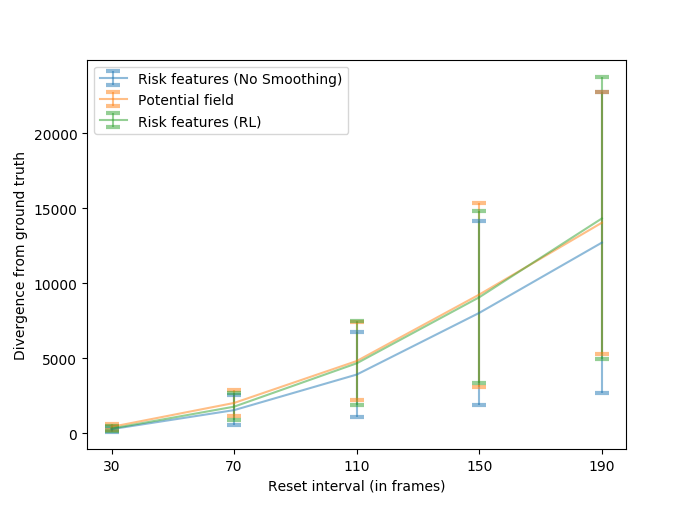
\includegraphics[width=\linewidth]{plots/inter_method/drift_analysis_easy.png}
		\caption {Drift analysis easy}
		\label{fig:inter_method-drift_analysis_easy}
	\end{subfigure}
	\begin{subfigure}{0.5\textwidth}
		\centering
		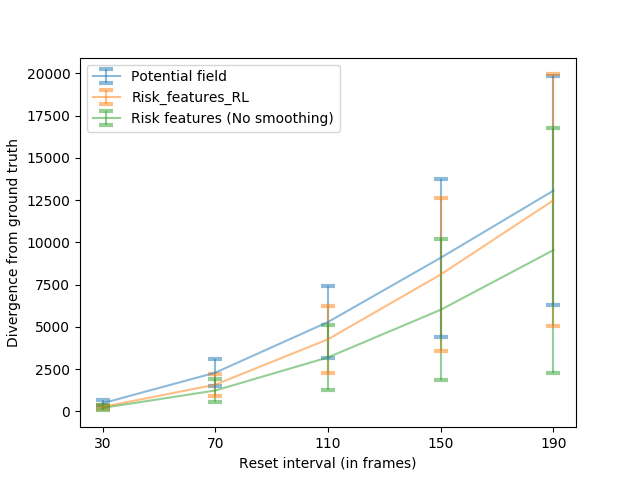
\includegraphics[width=\linewidth]{plots/inter_method/drift_analysis_med.png}
		\caption {Drift analysis medium}
		\label{fig:inter_method-drift_analysis_med}
	\end{subfigure}
	\begin{subfigure}{0.5\textwidth}
		\centering
		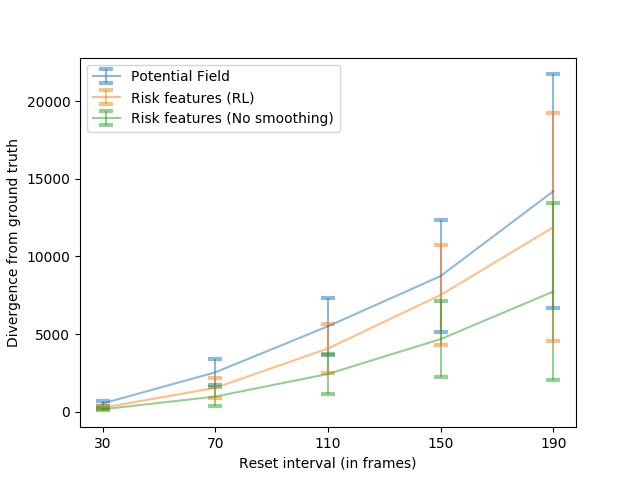
\includegraphics[width=\linewidth]{plots/inter_method/drift_analysis_hard.png}
		\caption {Drift analysis hard}
		\label{fig:inter_method-drift_analysis_hard}
	\end{subfigure}
	\begin{subfigure}{0.5\textwidth}
		\centering
		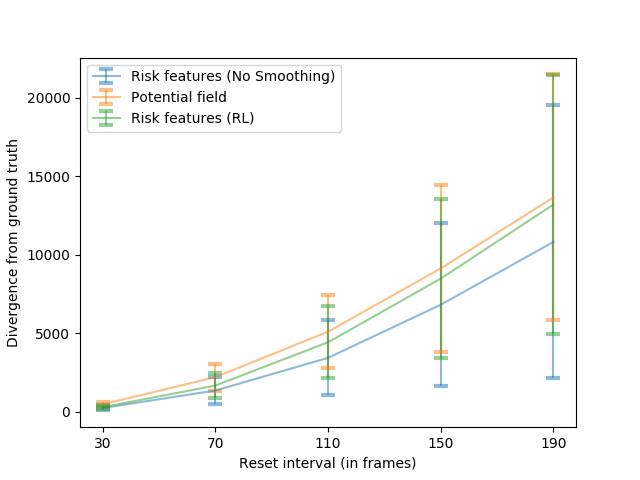
\includegraphics[width=\linewidth]{plots/inter_method/drift_analysis_all.png}
		\caption {Drift analysis all}
		\label{fig:inter_method-drift_analysis_all}
	\end{subfigure}
	\caption{Drift analysis}
\end{figure}


\subsection*{Testing the performance of our feature representation against pre-existing ones}
\subsubsection*{Description of the other feature extractors}
To test for the efficacy of our proposed risk-based feature representation, we test agents trained on our training pipeline with different existing feature representations. For this, we use feature representations proposed in \cite{fahadLearningHowPedestrians2018a} and \cite{vasquezInverseReinforcementLearning2014a} with some minor modifications and adjustments.\\
\textbf{Fahad}\\
Due to an underwhelming performance of the originally proposed SAM feature representation from \cite{fahadLearningHowPedestrians2018a} in our environmental setup, we substitute the part of the feature representation accommodating the goal information originally proposed by the authors with our goal representation. We call this modified version the 'Goal conditioned SAM'.\\
\textbf{Vasquez}\\
We use the feature sets $\mathcal{F}_1$, $\mathcal{F}_2$ and $\mathcal{F}_3$ from \cite{vasquezInverseReinforcementLearning2014a} and as before substitute their goal information with our goal information.
To compare against the risk features, we pick the feature set $\mathcal{F}_3$, which performed the out best of the three representations in our tests.\\
\textbf{Discuss the results}
\begin{figure}[!htbp]
	\begin{subfigure}{.5\textwidth}
		\centering
		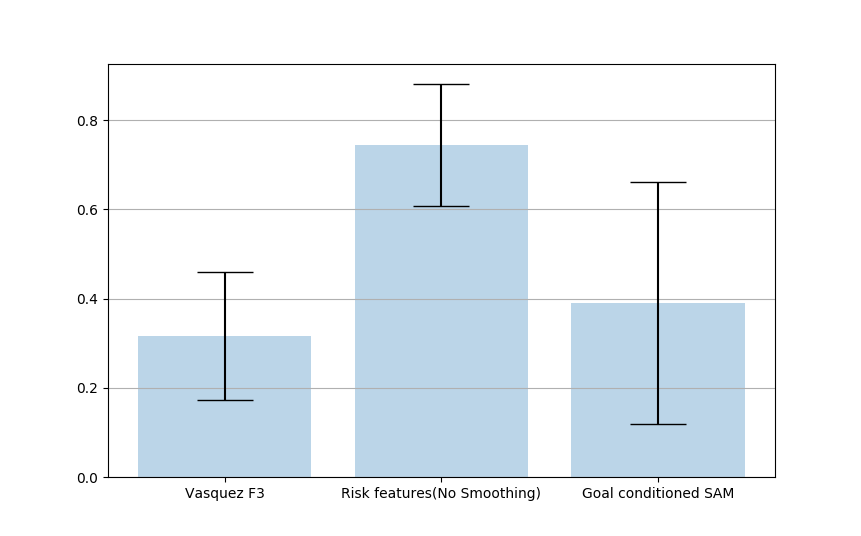
\includegraphics[width=\linewidth, height=6cm]{plots/inter_IRL/goal_reached.png}
		\label{fig:inter_IRL-goal_reached}
		\caption{Fraction of the runs in which the agent successfully reaches the goal}
	\end{subfigure}
	\begin{subfigure}{.5\textwidth}
		\centering
		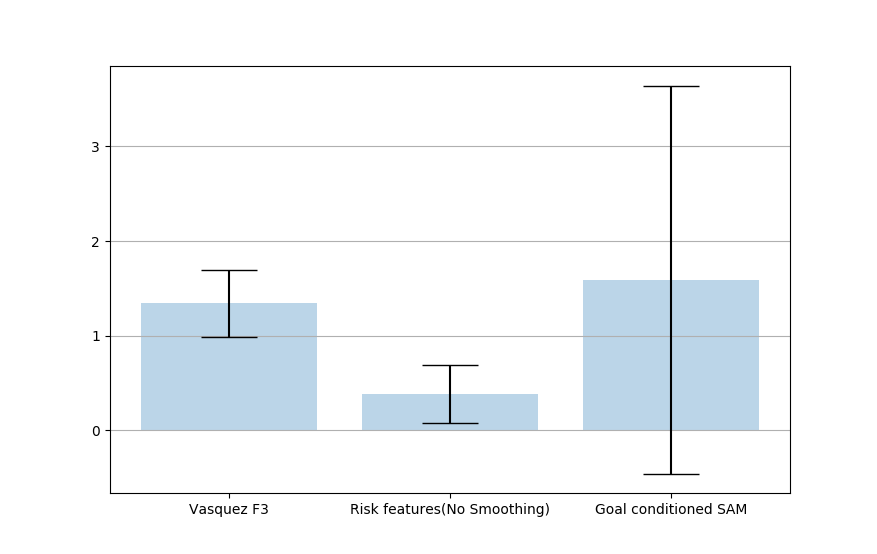
\includegraphics[width=\linewidth, height=6cm]{plots/inter_IRL/count_collisions.png}
		\label{fig:inter_IRL-collision_counts}
		\caption{Average number of collisions encountered by the agent per trajectory.}
	\end{subfigure}
	\caption{Comparing the fundamental requirements for navigation of different feature representations }
\end{figure}

\begin{figure}[htbp]
	\centering
	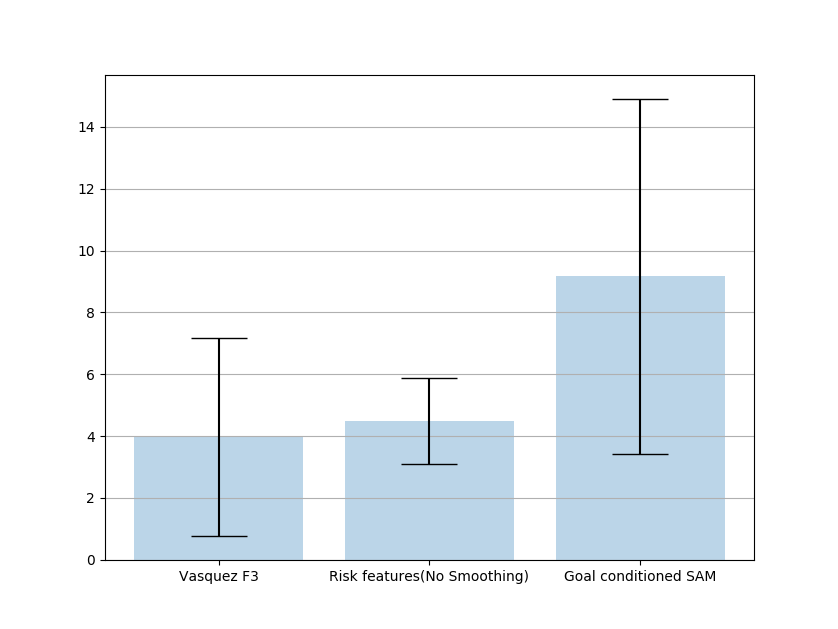
\includegraphics[width=0.7\linewidth]{plots/inter_IRL/avg_trajectory_smoothness.png}
	\caption{Average change in orientation of different agents.}
	\label{fig:inter_IRL-change_in_orientation_avg}
\end{figure}

\begin{figure}[htbp]
	\begin{subfigure}{\textwidth}
		\centering
		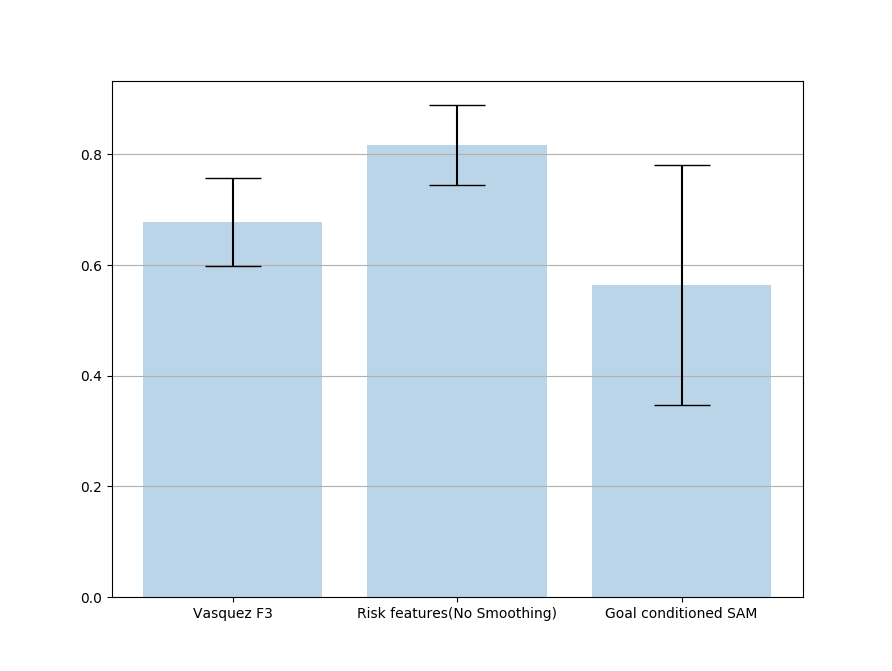
\includegraphics[width=.7\linewidth]{plots/inter_IRL/distance_displacement_ratio_barplots.png}
		\caption{Histogram plot of distance displacement ratio.}
		\label{fig:inter_IRL-distance_disp_ratio}
	\end{subfigure}
	\begin{subfigure}{\textwidth}
		\centering
		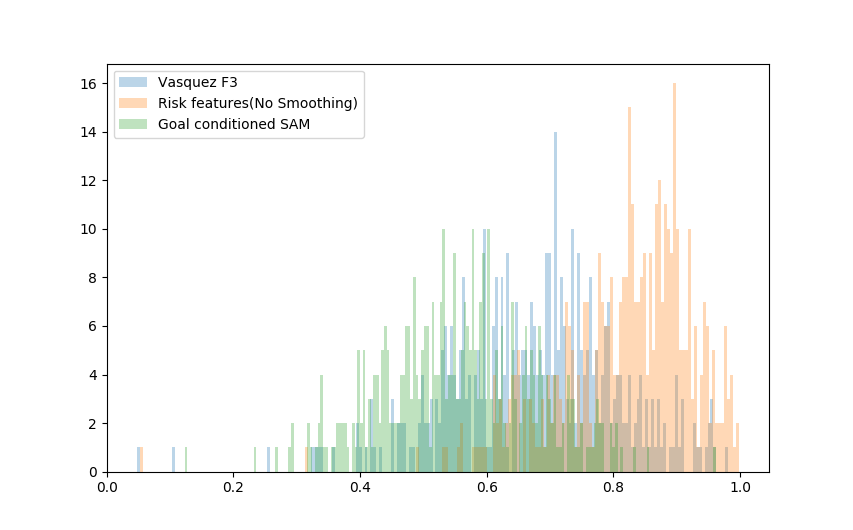
\includegraphics[width=.95\linewidth]{plots/inter_IRL/distance_displacement_ratio_histplot.png}
		\caption{Histogram plot of distance displacement ratio.}
		\label{fig:inter_IRL-distance_disp_ratio_histplot}
	\end{subfigure}
	\caption{Comparing the efficiency of the path taken by the different agents to reach their goals}
\end{figure}

We carry out a similar performance analysis as before. Figure \ref{fig:inter_IRL-goal_reached} and \ref{fig:inter_IRL-collision_counts} show that in both the fundamental tasks, the risk features outperforms the others with a considerable margin, reaching the goal $74.49\%$ of the times as compared to $31.59\%$ and $38.98\%$ of Vasquez $\mathcal{F}3$ and Goal Conditioned SAM respectively and encountering significantly less collision counts, $0.39$, as compared to $1.34$ and $1.59$ from the other two representations. In qualitative evaluation metrics, the risk feature based agent produces comparable results in terms of trajectory smoothness (Figure. \ref{fig:inter_IRL-change_in_orientation_avg}), and outperforms the others at making efficient navigation choices producing shorter paths to the goal while avoiding obstacles (Figure. \ref{fig:inter_IRL-distance_disp_ratio_histplot}). Table \ref{tab:inter_irl_numerical_comparison} summarizes the scores obtained by the different feature representations.
\begin{table}[htbp]
	\begin{center}
		\renewcommand{\arraystretch}{1.3}
		\begin{tabular}{|c|c|c|c|}
			\hline
			Metric Name & Risk Features & Goal augmented  & Vasquez $\mathcal{F}3$ \ \\
			  &   & SAM  &  \\
			\hline
			Goal reached (in $\%$) & $74.49$ & $38.98$ & $31.59$ \\
			Collisions encountered (per run) & $0.38$ & $1.59$ & $1.34$ \\
			Change in orientation ( $\degree$ per frame) & $4.48$ & $9.17$ &  $3.98$\\
			Displacement to Distance ratio & $0.81$ &  $0.56$ & $0.67$\\
			\hline
		\end{tabular}
	\end{center}
	\caption{Score obtained by the different feature representations across different metrics}
	\label{tab:inter_irl_numerical_comparison}
\end{table}\\

%drift analysis
\begin{figure}[htbp]
	\begin{subfigure}{0.5\textwidth}
		\centering
		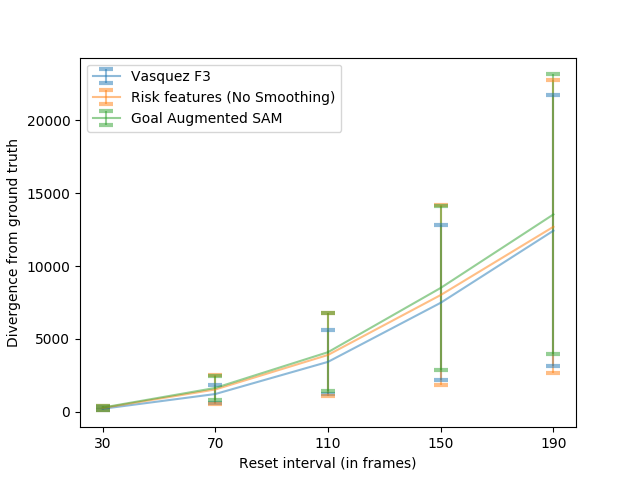
\includegraphics[width=\linewidth]{plots/inter_IRL/drift_analysis_easy.png}
		\caption {Drift analysis easy}
		\label{fig:inter_IRL-drift_analysis_easy}
	\end{subfigure}
	\begin{subfigure}{0.5\textwidth}
		\centering
		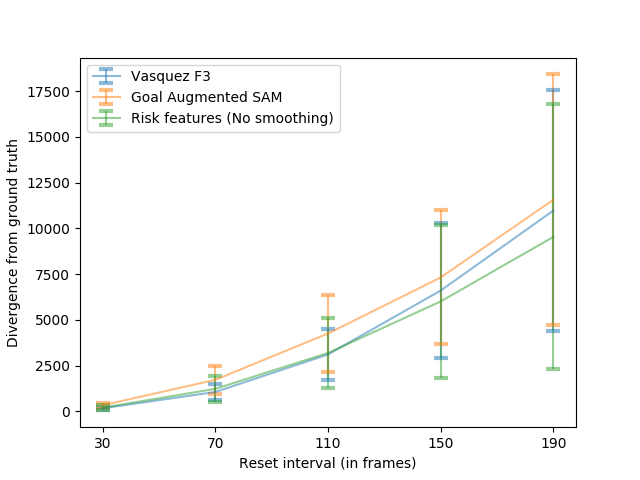
\includegraphics[width=\linewidth]{plots/inter_IRL/drift_analysis_med.png}
		\caption {Drift analysis medium}
		\label{fig:inter_IRL-drift_analysis_med}
	\end{subfigure}
	\begin{subfigure}{0.5\textwidth}
		\centering
		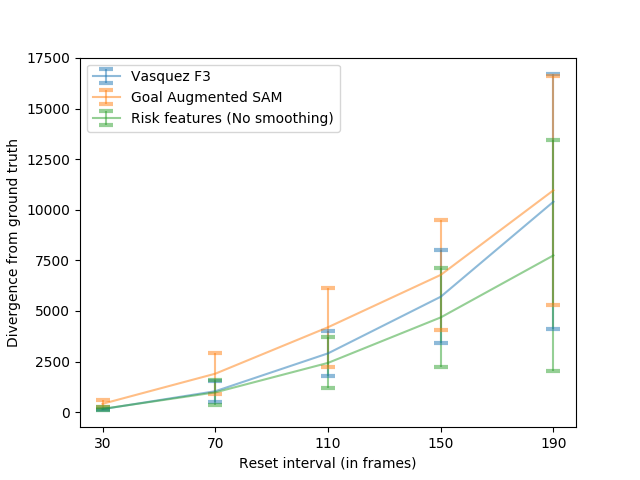
\includegraphics[width=\linewidth]{plots/inter_IRL/drift_analysis_hard.png}
		\caption {Drift analysis hard}
		\label{fig:inter_IRL-drift_analysis_hard}
	\end{subfigure}
	\begin{subfigure}{0.5\textwidth}
		\centering
		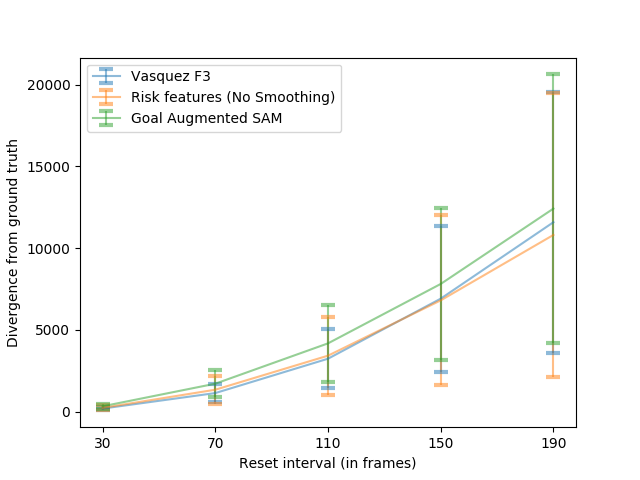
\includegraphics[width=\linewidth]{plots/inter_IRL/drift_analysis_all.png}
		\caption {Drift analysis all}
		\label{fig:inter_IRL-drift_analysis_all}
	\end{subfigure}
	\caption{Drift analysis inter IRL}
\end{figure}
The difference is less pronounced as compared to the agents from different methods(Figures. \ref{fig:inter_IRL-drift_analysis_all}, \ref{fig:inter_IRL-drift_analysis_easy}, \ref{fig:inter_IRL-drift_analysis_med}), with the Vasquez $\mathcal{F}3$ outperforming the risk features in the lower level of difficulty, the Risk feature based agent catches up and outperforms the existing feature representations, at the higher levels(Figure. \ref{fig:inter_IRL-drift_analysis_hard}.)

\subsection*{Testing for generalization}
Description of the other dataset.
Discussion of the results.
\subsection*{Testing on custom scenarios}
\textbf{Follow the group}
follow\_the\_group\_1.txt(subject 5)
follow\_the\_group\_3.txt(subject 2)
\textbf{Passing}

\textbf{t-junctions}

\textbf{avoiding group}

\subsection*{Understanding the reward function}
Something that is mostly forgotten if you look at most of the navigation related work. They never discuss the results.
